\documentclass[aspectratio=169]{beamer}

\mode<presentation> {
\usetheme{Goettingen}
\setbeamertemplate{footline}
}

\usepackage{mathabx} % astronomical symbols
\usepackage{wrapfig}
\usepackage{graphicx}
\usepackage{booktabs}
\usepackage{sidecap}
\usepackage{caption}

\title[Exoplanets detection methods and results]{Exoplanets detection methods and results}

\author{}
\date{}

\begin{document}

{
\setbeamertemplate{navigation symbols}{}
\usebackgroundtemplate{%
\vbox to \paperheight{\vfil\hbox to \paperwidth{\hfil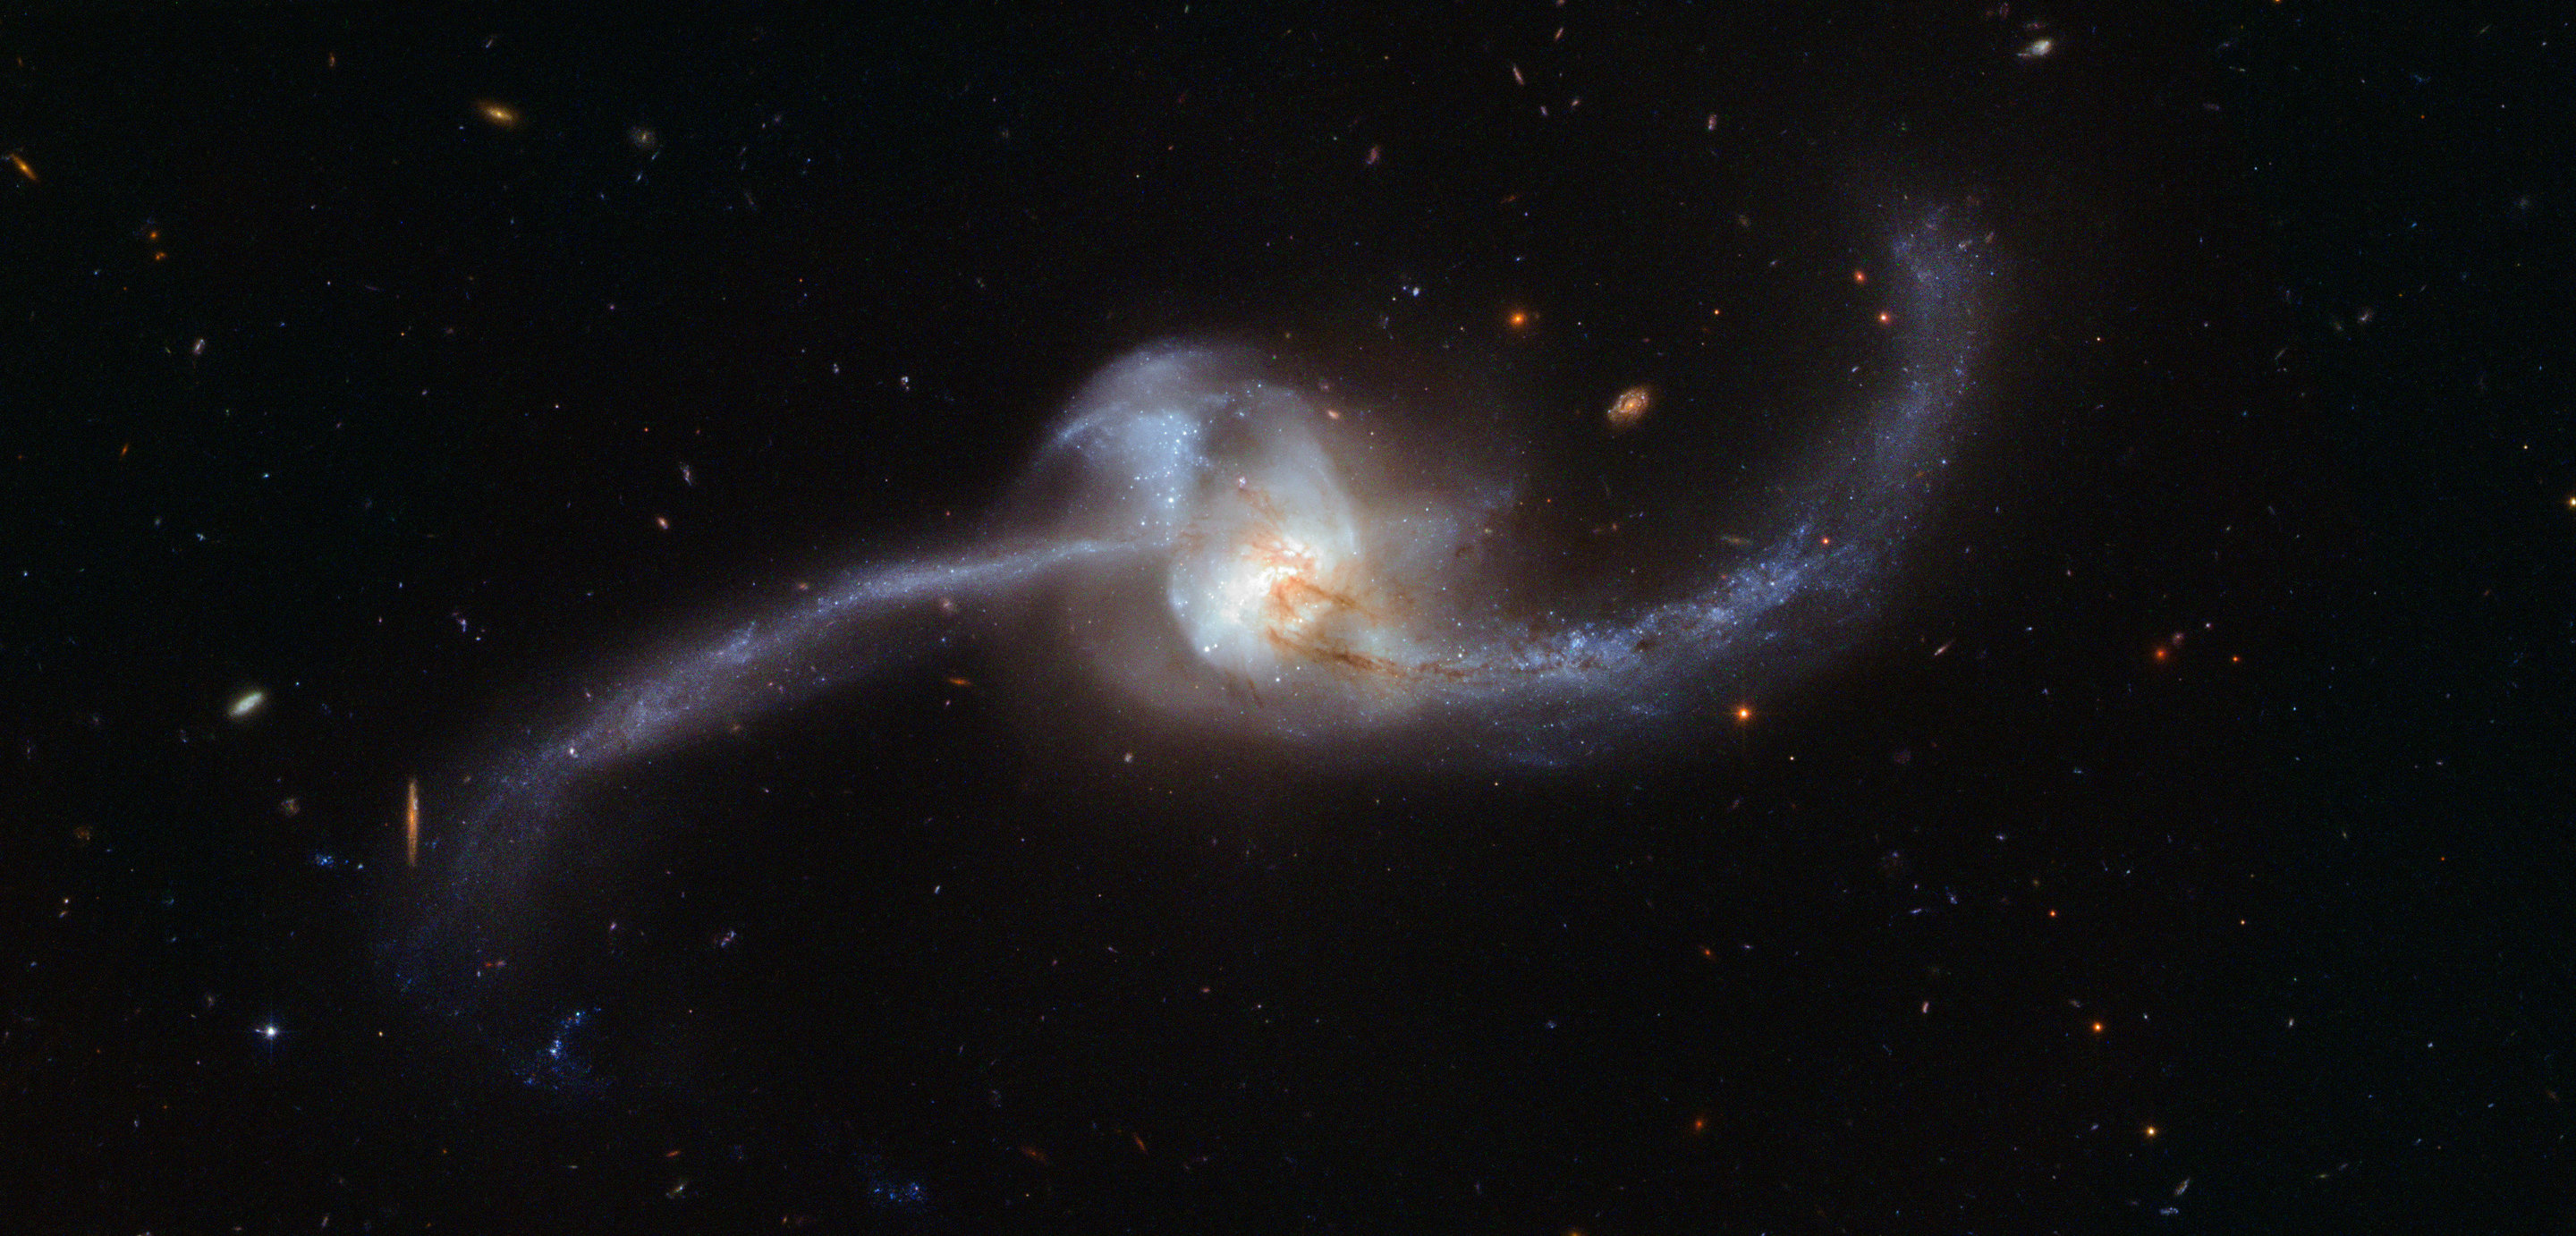
\includegraphics[width=\paperwidth]{img/NGC2623.jpg}\hfil}\vfil}
}
\begin{frame}[plain]
\vspace{-5.7cm}
\small{
\centerline{There are also numberless earths circling around their suns...}
}
\end{frame}
}

\begin{frame}
\frametitle{Agenda}
\tableofcontents
\end{frame}

\section{Brief review of results}
\begin{frame}
\frametitle{Exoplanets: brief review of results}
\begin{block}{Exoplanet}
Extrasolar planet is a planet located outside the Solar system
\end{block}
\begin{itemize}
\item $\approx 4050$ confirmed planets as of April 2019 \cite{exoplanet.eu}
\item $\approx 50$ {\bf potentially} habitable planets
\item Known parameters: orbital period, distance to the star, mass
\item Only a handful of direct observations
\end{itemize}
\end{frame}

\section{History of exoplanets exploration}
\begin{frame}
\frametitle{History of exoplanets exploration}
\begin{itemize}
\item 1584 "Innumerable suns and earths" hypothesis by Giordano Bruno
\item 1992 $M_\Earth$ planet orbiting \href{https://en.wikipedia.org/wiki/PSR_B1257\%2B12}{PSR B1257+12} pulsar
\item 1995 Planet orbiting a main sequence star detected by
      \href{http://www.obs-hp.fr/guide/elodie/elodie-eng.html}{ELODIE spectrograph}
\item 2008 30+ planets discovered by \href{http://www.eso.org/sci/facilities/lasilla/instruments/harps.html}{HARPS spectrograph}
\item 2014 Discovery of 715 planets around 305 stars by %
      \href{http://www.nasa.gov/mission_pages/kepler/main/index.html}{Kepler Space Telescope}
\end{itemize}
\end{frame}

\section{Methods of detection}
\begin{frame}
\frametitle{Methods of detection}
\begin{columns}
\column{0.25\textwidth}
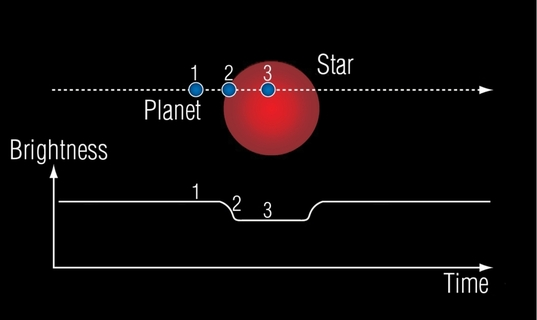
\includegraphics[width=0.90\textwidth]{img/20130108_Planetary_transit_f537.jpg}
\column{0.75\textwidth}
\begin{block}{Transit photometry}
As the planet moves in front of its star the star luminosity dips, and then returns to its former level
\end{block}
\end{columns}

\begin{columns}
\column{0.25\textwidth}
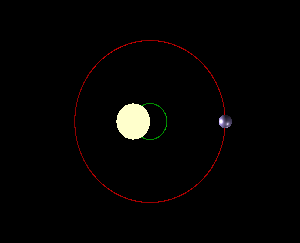
\includegraphics[width=0.90\textwidth]{img/Dopplerspectr-above.png}
\column{0.75\textwidth}
\begin{block}{Doppler spectroscopy}
Star moves in a small circle when it is orbited by a planet. These movements causes
a tiny periodic Doppler shift 
\end{block}
\end{columns}
\begin{block}{Others}
\begin{itemize}
\item Direct infrared imaging (young hot heavy planets)
\item Gravitational microlensing
\item Precision measurement of stars' location
\end{itemize}
\end{block}
\end{frame}

\section{Transit photometry}
\begin{frame}
\frametitle{Transit photometry}

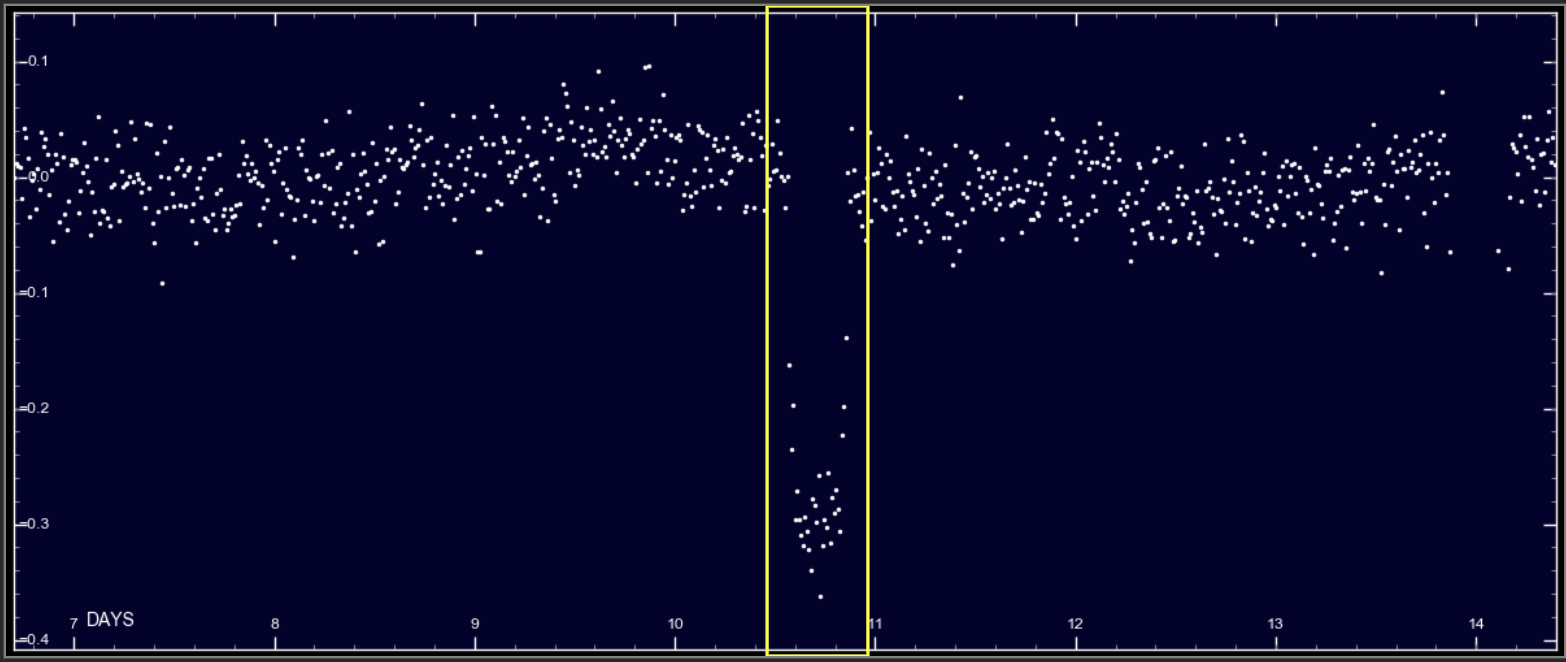
\includegraphics[width=0.35\textwidth]{img/zooniverse.org/obvious_transit.png}

\begin{itemize}
\item[+] Planet size estimates (not available with other methods)
\item[+] Atmosphere composition (due to absorption spectrum)
\item[+] Massively scalable ($\sim 10^5$ stars at a time)
\item[-] Planet must pass directly between its star and Earth
\item[-] Transits are very short (last hours or days)
\item[-] False positives due to eclipsing binaries, stellar variability
\end{itemize}
\end{frame}

\begin{frame}
\frametitle{Examples of transits}
\begin{columns}[c]

\column{0.48\textwidth}
\begin{figure}
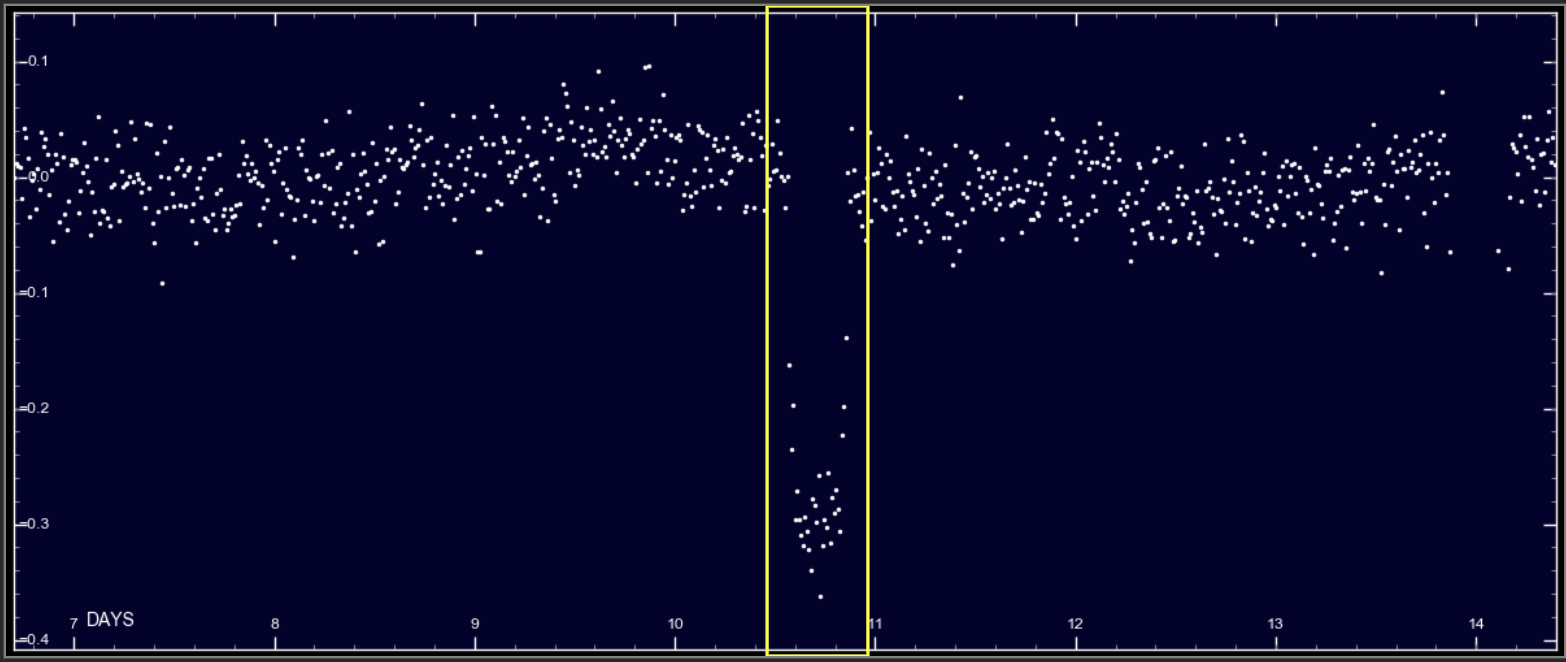
\includegraphics[height=0.24\textheight]{img/zooniverse.org/obvious_transit.png}
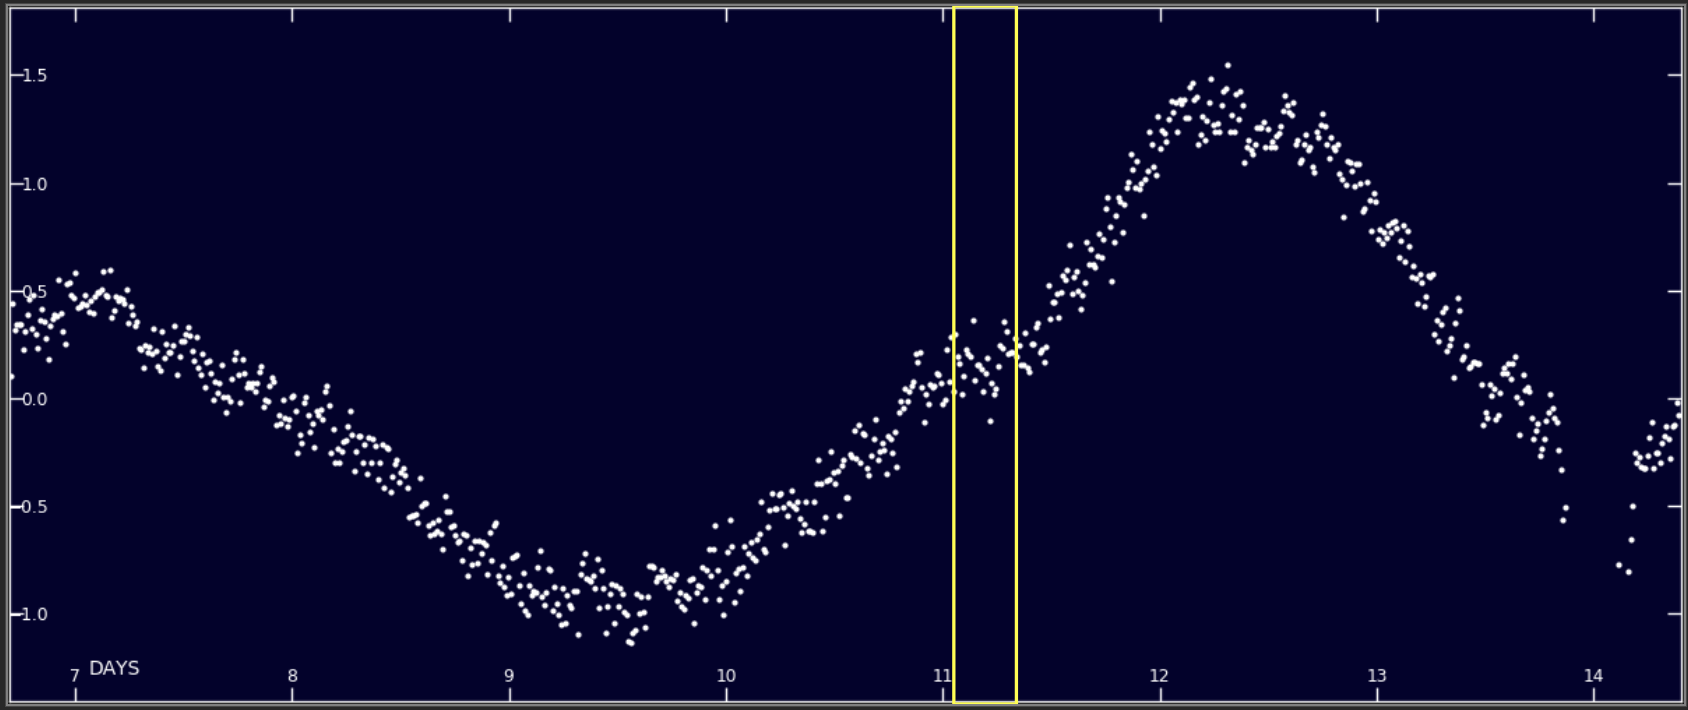
\includegraphics[height=0.24\textheight]{img/zooniverse.org/shallow_transit.png}
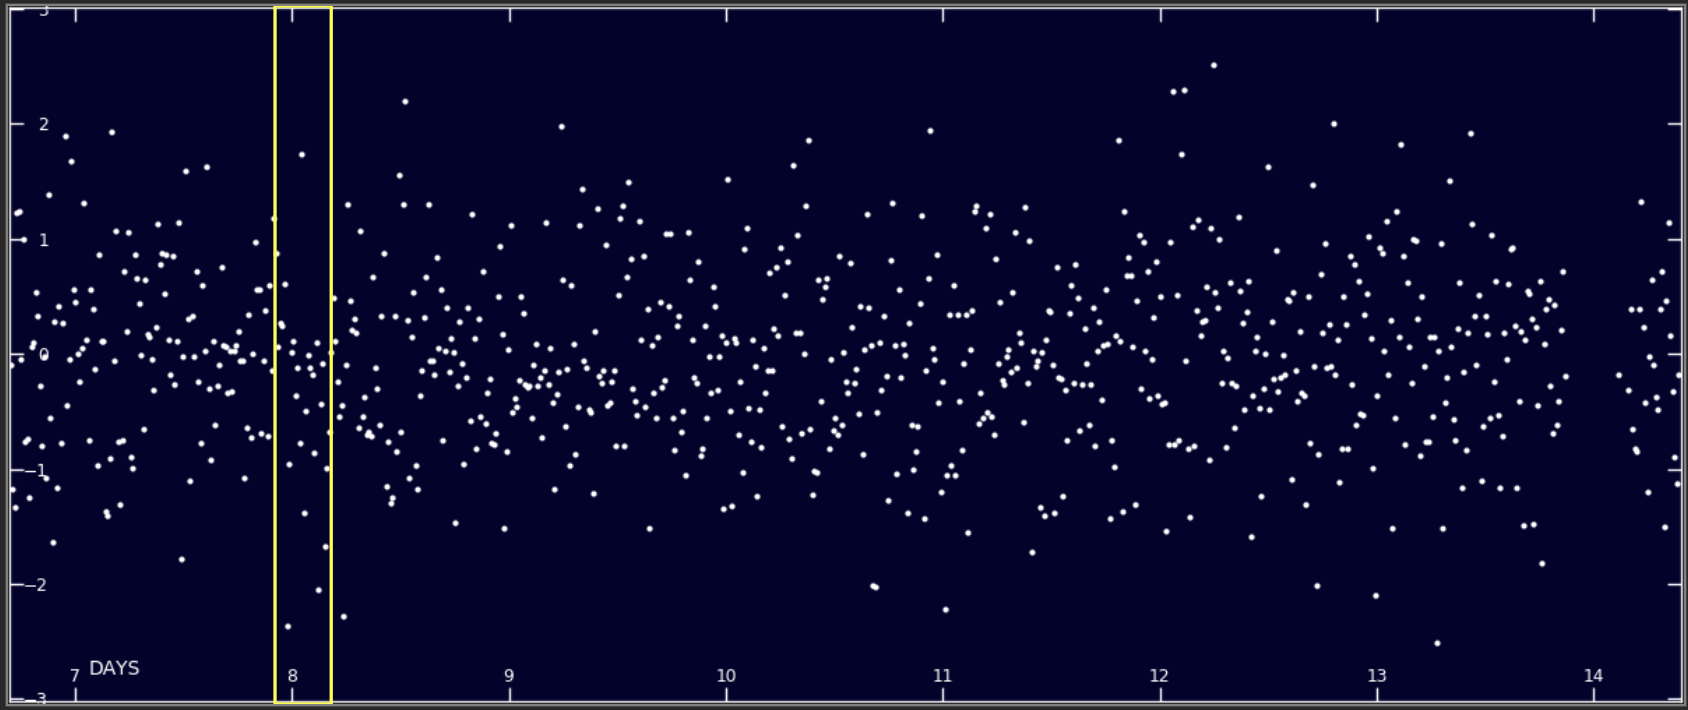
\includegraphics[height=0.24\textheight]{img/zooniverse.org/stellar_variability_transit.png}
\captionsetup{labelformat=empty}
\onslide<2->{\caption{Genuine transits}}
\end{figure}

\column{0.48\textwidth}
\begin{figure}
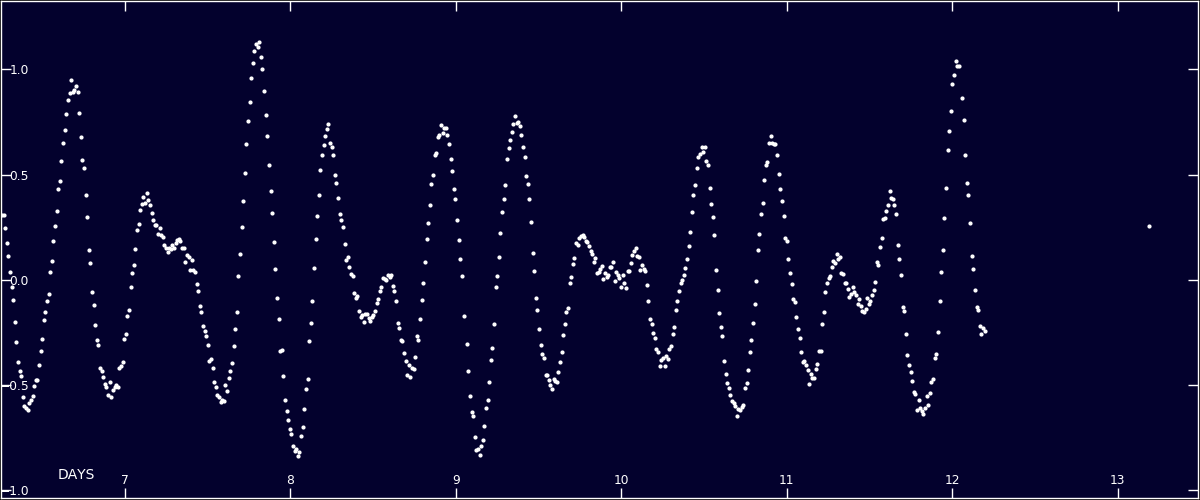
\includegraphics[height=0.24\textheight]{img/zooniverse.org/starspots_moderate.png}
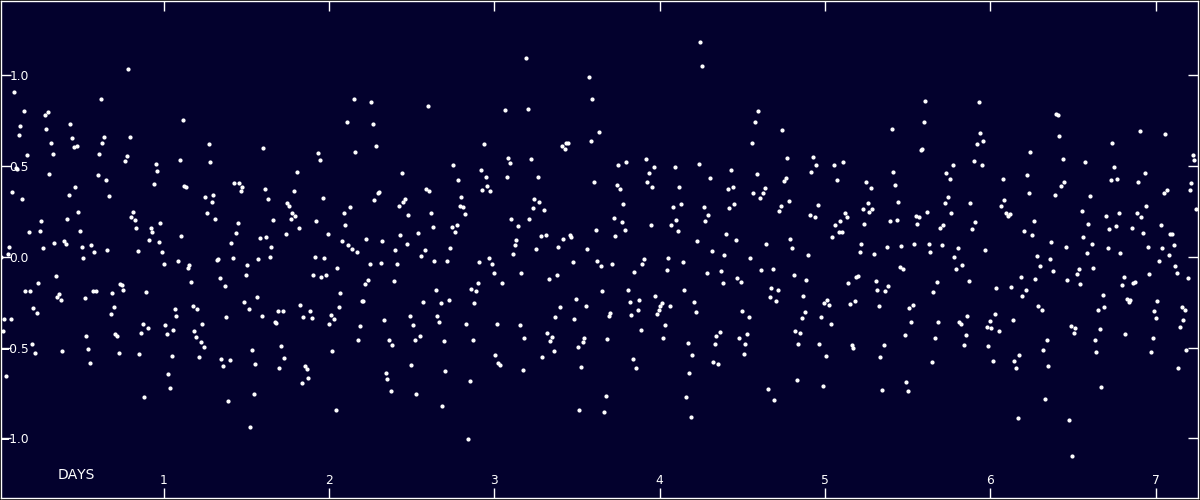
\includegraphics[height=0.24\textheight]{img/zooniverse.org/startspots_fast.png}
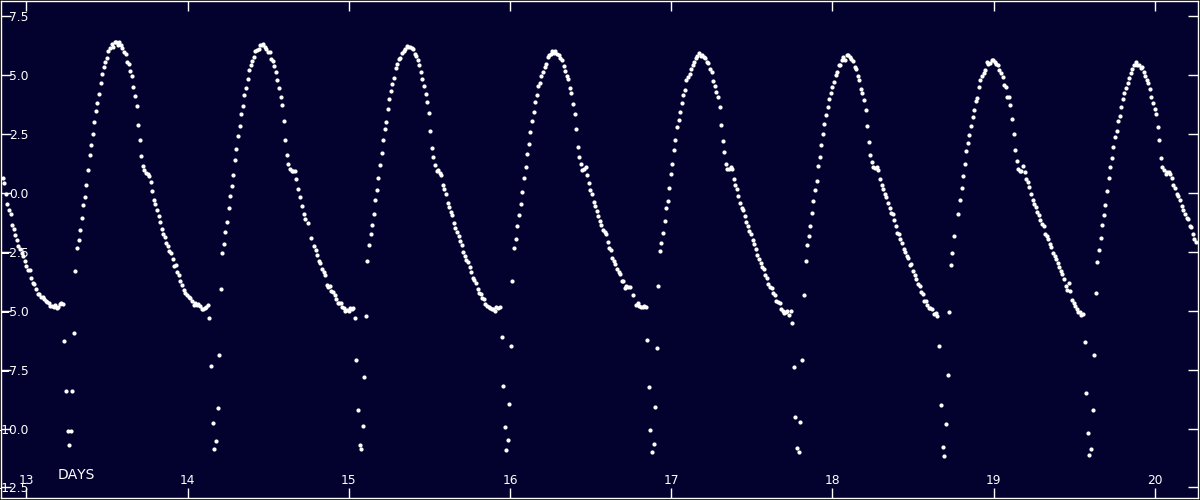
\includegraphics[height=0.24\textheight]{img/zooniverse.org/eclipsing_binaries_another.png}
\captionsetup{labelformat=empty}
\onslide<2->{\caption{Star spots, eclipsing binaries}}
\end{figure}
\end{columns}
\end{frame}

\begin{frame}
\frametitle{Transit photometry: instruments}
\begin{itemize}
\item
Kepler Space Telescope, April 2009 -- October 2018
\begin{itemize}
\item 530000+ stars observed
\item 2600+ exoplanets detected
\end{itemize}
\item
Transiting Exoplanet Survey Satellite (TESS), April 2018 -- now
\begin{itemize}
\item Study 500000 stars across the whole sky, including 1000 closest red dwarfs
\item Discover $\sim 20000$ exoplanets, including 500 -- 100 Earth-sized ones
\item At least 5 exoplanets discovered as of April 15, 2019
\end{itemize}
\end{itemize}

\end{frame}


\section{Doppler spectroscopy}
\begin{frame}
\frametitle{Doppler spectroscopy}

\begin{columns}
\column{0.75\textwidth}
Sun: orbital speed: $V_{orb} \approx 200 \mathrm{km/s}$ \\
Radial velocity of Sun due to Jupiter: $\approx 12.7 m/s$ \\
\begin{itemize}
\item[+] 1st method that worked with main sequence stars
\item[+] Good at detecting "hot Jupiter" planets
\item[-] Earth like planets undetectable with current instruments
\item[-] Only the lower bound of mass can be estimated
\item[-] False positives due to intrinsic variability of stars
\item[-] No Doppler shift if the orbital plane is "edge-on"
\end{itemize}
\column{0.25\textwidth}
\begin{figure}
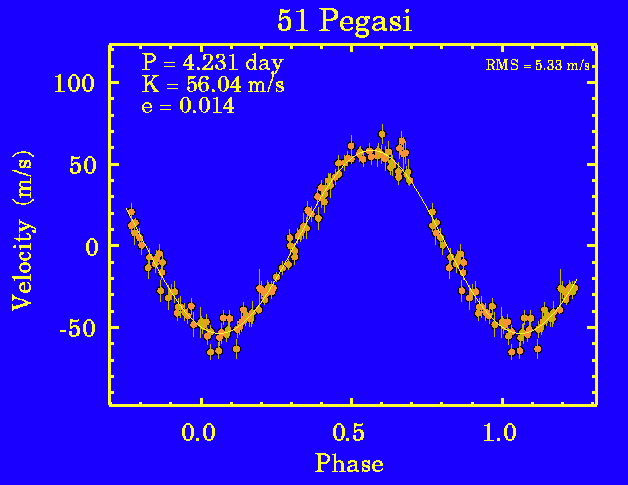
\includegraphics[width=\textwidth]{img/51Pegasi.png}
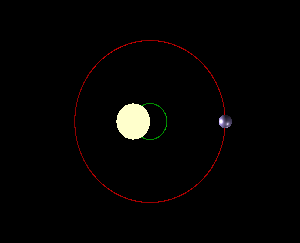
\includegraphics[width=\textwidth]{img/Dopplerspectr-above.png}
\end{figure}

\end{columns}
\end{frame}

\begin{frame}
\frametitle{Doppler spectroscopy: instruments}
\begin{block}{\href{http://www.obs-hp.fr/guide/elodie/elodie-eng.html}{ELODIE Spectrograph} (1993 -- 2006)}
Discovered 1st exoplanet orbiting an ordinary star. \\
Resolution: $\sim 10 \: \mathrm{m/s}$
\end{block}
\begin{block}{\href{https://www.eso.org/sci/facilities/lasilla/instruments/harps.html}{%
HARPS Spectrograph} (2003 -- now)}
Discovered 130+ exoplanets. \\
Resolution: $\sim 1 \: \mathrm{m/s}$
\end{block}
\begin{block}{\href{https://www.eso.org/sci/facilities/paranal/instruments/espresso.html}{%
ESPRESSO Spectrograph} (under construction)}
Capable of detecting Earth-like planets. \\
Resolution (planned): $\sim 0.1 \: \mathrm{m/s}$
\end{block}
\end{frame}

\section{Summary}
\begin{frame}
\frametitle{Summary}
\begin{itemize}
\item $\sim 4000$ confirmed exoplanets as of April 2019
\item Planets outnumber stars
\item Small planets are common (around 20 -- 50\% of stars)
\item Several atmospheres of "hot Jupiters" have been detected
\item 1st atmosphere of Earth-sized planet discovered in 2016 \cite{arXiv:1612.02425}
\end{itemize}
\end{frame}

\begin{frame}
\frametitle{Any aliens?}
\begin{itemize}
\item 49 potentially habitable planets discovered
\begin{itemize}
\item {\bf Likely} to have a rocky composition
\item {\bf Likely} to maintain surface liquid water
\end{itemize}
\item Atmospheres' composition haven't been measured yet
\item No estimates of the surface temperature
\item No artificial structures have been detected
\end{itemize}
\begin{block}{What about \href{http://en.wikipedia.org/wiki/KIC_8462852}{Tabby's star}?}
Unusual dimming (up to 21\%) is caused by dust \cite{arXiv:1809.00693}
\end{block}
\end{frame}

\section{References}
\begin{frame}[allowframebreaks]
\footnotesize{


\begin{thebibliography}{99}

\bibitem{exoplanet.eu}The Extrasolar Planets Encyclopaedia
\newblock \href{http://exoplanet.eu}{exoplanet.eu}

\bibitem{arXiv:1612.02425}John Southworth, Luigi Mancini, Nikku Madhusudhan, Paul Molliere, Simona Ciceri, Thomas Henning
\newblock Detection of the atmosphere of the 1.6 Earth mass exoplanet GJ 1132b
\newblock \href{http://arxiv.org/abs/1612.02425}{arXiv:1612.02425}

\bibitem{arXiv:1809.00693}Jason T. Wright
\newblock A Reassessment of Families of Solutions to the Puzzle of Boyajian's Star
\newblock \href{https://arxiv.org/abs/1809.00693}{arXiv:1809.00693}
\end{thebibliography}
}
\end{frame}


\end{document}
